\documentclass[a4paper,11pt]{article}
\usepackage[utf8]{inputenc}
\usepackage[T1]{fontenc}
\usepackage[english]{babel}
\usepackage{lmodern}
\usepackage{microtype}
\usepackage{amsmath,amssymb,bm,mathtools}
\usepackage{geometry}
\geometry{a4paper, left=2.4cm, right=2.4cm, top=2.0cm, bottom=2.2cm}
\usepackage{booktabs,multirow,array}
\usepackage{xcolor}
\definecolor{bokug}{RGB}{0,135,60}
\usepackage{tikz}
\usetikzlibrary{patterns,arrows.meta,calc,decorations.pathmorphing,
                 decorations.markings}
\usepackage{fancyhdr}
\pagestyle{fancy}
\renewcommand{\headrulewidth}{0.4pt}
\renewcommand{\footrulewidth}{0.4pt}
\usepackage{enumitem}
\setlength{\parindent}{0pt}
\setlength{\parskip}{4pt}
\begin{document}

\fancyhead[L]{\small VU Mechanics -- LAWI 100515 (PI)\quad SS 2026}
\fancyhead[R]{\small 2nd Exercise Exam\quad 26.06.2026\quad Group~A}
\fancyfoot[C]{\small 26.06.2026 \qquad Mechanics VU -- LAWI 100515 (PI) \qquad SS 2026}
\fancyfoot[R]{\small Page~\thepage}

\begin{center}
  {\LARGE\bfseries VU MECHANICS -- LAWI 100515 (PI)\\[4pt]
  SS 2026}\\[10pt]
  {\Large\bfseries 2nd Exercise Exam}\\[4pt]
  {\large 26.06.2026 \quad GROUP~A}
\end{center}

\vspace{6pt}
\begin{center}
\begin{tabular}{|p{4.5cm}|p{8cm}|}
\hline
Name: & \\[8pt] \hline
Student ID number: & \\[8pt] \hline
Study program code: & \\[8pt] \hline
Notes & \\[14pt] \hline
\multicolumn{1}{|l|}{Result} & \hspace{3cm}\_\_\_/100 \\[6pt] \hline
\end{tabular}
\end{center}

\vspace{6pt}
\begin{tabular}{lcc}
\toprule
\textbf{Tasks} & \textbf{Possible Points} & \textbf{Achieved Points} \\
\midrule
1)\;Task 1 -- Section Forces and Moments & 40 & \\
2)\;Task 1 -- Truss System               & 30 & \\
3)\;Task 2                               & 30 & \\
\bottomrule
\end{tabular}

\medskip
\textbf{Working Time:} 90~min\quad
\textbf{Passing Grade:} $\geq 50\,\%$

\textbf{Permitted Aids:} Formula sheet (boku-learn), calculator, set square, compass.
No pencil, no red pen, no own paper.

\newpage
\section*{1.~Task \hfill (70\,\%)}

\textbf{Given} is the planar static system shown below.
Dimensions and system parameters are given in the sketch.
The structure is loaded by a \textbf{\textcolor{blue!70!black}{uniformly distributed load~$q$}}
acting on beams [1] and [2], and a
\textbf{\textcolor{red!70!black}{concentrated load~$P$}} at truss node~D.

\medskip
\begin{tabular}{|c|c|c|}
\hline
$L = 0.5$\,m & $q = 2$\,kN/m & $P = 20$\,kN \\
\hline
\end{tabular}


\begin{center}
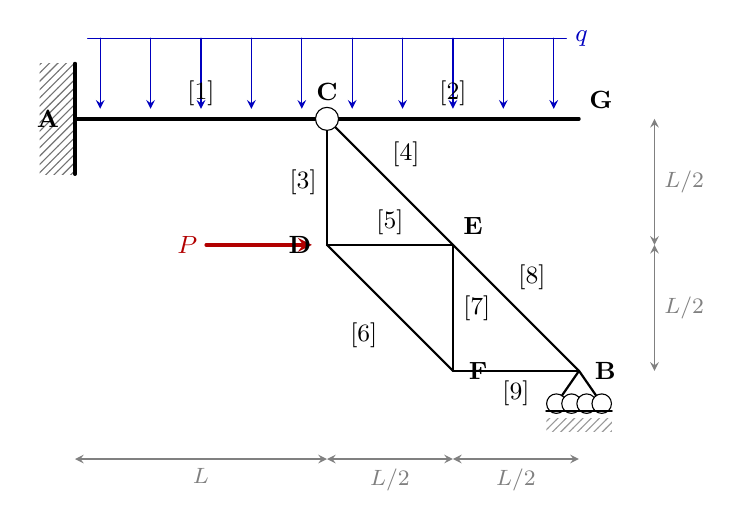
\begin{tikzpicture}[scale=3.2, >=stealth, line cap=round, line join=round,
    thick, font=\small]

  %--- Node coordinates (normalized: 1 unit = L) ----------------------------
  \coordinate (A)   at (0.00, 0.00);
  \coordinate (C)   at (1.00, 0.00);
  \coordinate (G)   at (2.00, 0.00);
  \coordinate (D)   at (1.00,-0.50);
  \coordinate (E)   at (1.50,-0.50);
  \coordinate (Fnd) at (1.50,-1.00);
  \coordinate (B)   at (2.00,-1.00);

  %--- Fixed support (Einspannung) at A ------------------------------------
  \fill[pattern=north east lines, pattern color=black!55]
        (-0.14,-0.22) rectangle (0.00, 0.22);
  \draw[very thick] (0,-0.22) -- (0, 0.22);

  %--- Beam members [1] and [2] --------------------------------------------
  \draw[very thick] (A) -- (G);

  %--- Truss members -------------------------------------------------------
  \draw (C) -- (D);         % [3]
  \draw (C) -- (E);         % [4]
  \draw (D) -- (E);         % [5]
  \draw (D) -- (Fnd);       % [6]
  \draw (E) -- (Fnd);       % [7]
  \draw (E) -- (B);         % [8]
  \draw (Fnd) -- (B);       % [9]

  %--- Hinge at C (open circle) -------------------------------------------
  \filldraw[fill=white, draw=black, thin] (C) circle (1.3pt);

  %--- Roller support at B (verschiebliches Lager, vertical reaction) ------
  \draw (B) -- ++(0.09,-0.13) -- ++(-0.18, 0) -- cycle;
  \foreach \dx in {-0.09, -0.03, 0.03, 0.09}
    \filldraw[fill=white, draw=black, thin]
              ($(B)+(\dx,-0.13)$) circle (1.1pt);
  \draw[thick] ($(B)+(-0.13,-0.16)$) -- ++(0.26, 0);
  \fill[pattern=north east lines, pattern color=black!40]
       ($(B)+(-0.13,-0.19)$) rectangle ++(0.26,-0.05);

  %--- Distributed load q (downward arrows above beam) --------------------
  \foreach \xx in {0.10,0.30,0.50,0.70,0.90,1.10,1.30,1.50,1.70,1.90}
    \draw[->, thin, blue!75!black] (\xx, 0.32) -- (\xx, 0.04);
  \draw[thin, blue!75!black] (0.05, 0.32) -- (1.95, 0.32);
  \node[blue!75!black, right, inner sep=1pt] at (1.97, 0.32) {$q$};

  %--- Point load P at D (horizontal, rightward) --------------------------
  \draw[->, very thick, red!70!black]
        ($(D)+(-0.48,0)$) -- ($(D)+(-0.06,0)$);
  \node[red!70!black, left, inner sep=1pt] at ($(D)+(-0.50,0)$) {$P$};

  %--- Node labels ---------------------------------------------------------
  \node[left,  xshift=-2pt] at (A)   {\textbf{A}};
  \node[above, yshift= 3pt] at (C)   {\textbf{C}};
  \node[above right]        at (G)   {\textbf{G}};
  \node[left,  xshift=-2pt] at (D)   {\textbf{D}};
  \node[above right]        at (E)   {\textbf{E}};
  \node[right, xshift= 2pt] at (Fnd) {\textbf{F}};
  \node[right, xshift= 2pt] at (B)   {\textbf{B}};

  %--- Member labels -------------------------------------------------------
  \node[above]        at (0.50, 0.01) {[1]};
  \node[above]        at (1.50, 0.01) {[2]};
  \node[left]         at (1.00,-0.25) {[3]};
  \node[above right, xshift=-1pt] at (1.23,-0.23) {[4]};
  \node[above]        at (1.25,-0.50) {[5]};
  \node[below left, xshift=1pt]   at (1.23,-0.77) {[6]};
  \node[right]        at (1.50,-0.75) {[7]};
  \node[above right, xshift=-1pt] at (1.73,-0.72) {[8]};
  \node[below]        at (1.75,-1.00) {[9]};

  %--- Dimension lines -----------------------------------------------------
  \draw[<->, thin, gray] (0.00,-1.35) -- (1.00,-1.35)
        node[midway, below, font=\footnotesize] {$L$};
  \draw[<->, thin, gray] (1.00,-1.35) -- (1.50,-1.35)
        node[midway, below, font=\footnotesize] {$L/2$};
  \draw[<->, thin, gray] (1.50,-1.35) -- (2.00,-1.35)
        node[midway, below, font=\footnotesize] {$L/2$};
  \draw[<->, thin, gray] (2.30, 0.00) -- (2.30,-0.50)
        node[midway, right, font=\footnotesize] {$L/2$};
  \draw[<->, thin, gray] (2.30,-0.50) -- (2.30,-1.00)
        node[midway, right, font=\footnotesize] {$L/2$};

\end{tikzpicture}
\end{center}


\textbf{Tasks:}
\begin{enumerate}[leftmargin=*, label=\arabic*.]
  \item Check whether the system is statically determinate.
  \item Determine the support reactions \textbf{in general form as functions of $q$, $P$, and $L$}.
        Draw the reactions into the system sketch.
  \item Evaluate the support reactions for the given parameters:
        \[
          A_V = \hspace{2.5cm}
          A_H = \hspace{2.5cm}
          M_A = \hspace{2.5cm}
          B_V = \hspace{2.5cm}
        \]
  \item Determine the section forces $M(x)$, $V(x)$, and $N(x)$ in beams [1] and [2]
        \textbf{in general form as functions of $q$, $P$, and $L$}.
        Define the range of the running variable~$x$.
        Evaluate the functions at the beam start and end:

        \medskip
        \begin{tabular}{l cccccc}
        \toprule
         & \multicolumn{3}{c}{\textbf{Beam start}} & \multicolumn{3}{c}{\textbf{Beam end}} \\
        \cmidrule(lr){2-4}\cmidrule(lr){5-7}
         & $M$\,[kNm] & $V$\,[kN] & $N$\,[kN]
         & $M$\,[kNm] & $V$\,[kN] & $N$\,[kN] \\
        \midrule
        Beam [1] & & & & & & \\[6pt]
        Beam [2] & & & & & & \\
        \bottomrule
        \end{tabular}

  \item Draw the distributions $M(x)$, $V(x)$, and $N(x)$ and mark the characteristic values.

  \item Calculate the axial forces $S_8$ and $S_9$ using a \textbf{circular cut (Rundschnitt)
        at node~B}, in general form as a function of~$P$:
        \[
          S_8 = \hspace{3cm} S_9 = \hspace{3cm}
        \]

  \item Calculate the axial forces $S_4$, $S_5$, and $S_6$ using \textbf{Ritter's cut
        (Ritterschnitt)}, in general form as a function of~$P$:
        \[
          S_4 = \hspace{2.5cm} S_5 = \hspace{2.5cm} S_6 = \hspace{2.5cm}
        \]
\end{enumerate}

\newpage
\section*{2.~Task \hfill (30\,\%)}

\textbf{Given} is a simply supported beam (span~$L$)
with a triangular load (0 at~A, $q_0$ at~B).
The support reactions are $A_v = \tfrac{1}{6}q_0 L$ and $B_v = \tfrac{1}{3}q_0 L$.
The bending moment distribution is:
\[
  M(x) = -\frac{q_0}{6L}\,x^3 + \frac{q_0 L}{6}\,x
  \qquad (0 \le x \le L)
\]

\begin{tabular}{|c|c|}
\hline
$L = 0.5$\,m & $q_0 = 4$\,kN/m \\
\hline
\end{tabular}


\begin{center}
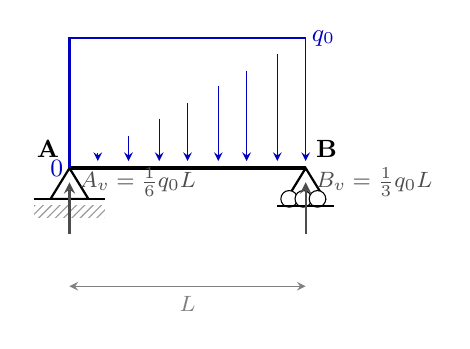
\begin{tikzpicture}[scale=3.0, >=stealth, thick, font=\small]

  \coordinate (A) at (0,0);
  \coordinate (B) at (1,0);

  %--- Beam ----------------------------------------------------------------
  \draw[very thick] (A) -- (B);

  %--- Pin support at A ----------------------------------------------------
  \draw (A) -- ++( 0.08,-0.13) -- ++(-0.16, 0) -- cycle;
  \draw[thick] ($(A)+(-0.15,-0.13)$) -- ++(0.30, 0);
  \fill[pattern=north east lines, pattern color=black!40]
       ($(A)+(-0.15,-0.16)$) rectangle ++(0.30,-0.05);

  %--- Roller support at B -------------------------------------------------
  \draw (B) -- ++(0.08,-0.13) -- ++(-0.16, 0) -- cycle;
  \foreach \dx in {-0.07, -0.01, 0.05}
    \filldraw[fill=white, draw=black, thin]
              ($(B)+(\dx,-0.13)$) circle (1.0pt);
  \draw[thick] ($(B)+(-0.12,-0.16)$) -- ++(0.24, 0);

  %--- Triangular load (0 at A, q0 at B) -----------------------------------
  \draw[blue!75!black] (A) -- ++(0, 0.55); % left edge (zero)
  \foreach \xx in {0.12, 0.25, 0.38, 0.50, 0.63, 0.75, 0.88, 1.00}
    \draw[->, thin, blue!75!black] (\xx, {0.55*\xx}) -- (\xx, 0.03);
  \draw[blue!75!black] (0,0) -- (0, 0.55) -- (1, 0.55);
  \node[blue!75!black, right, inner sep=1pt] at (1.01, 0.55) {$q_0$};
  \node[blue!75!black, left,  inner sep=1pt] at (-0.01, 0)   {$0$};

  %--- Node labels ---------------------------------------------------------
  \node[above left]  at (A) {\textbf{A}};
  \node[above right] at (B) {\textbf{B}};

  %--- Support reaction labels ---------------------------------------------
  \draw[->, thick, black!70]  ($(A)+(0,-0.28)$) -- ++(0, 0.22)
        node[right, font=\footnotesize] {$A_v = \frac{1}{6}q_0 L$};
  \draw[->, thick, black!70]  ($(B)+(0,-0.28)$) -- ++(0, 0.22)
        node[right, font=\footnotesize] {$B_v = \frac{1}{3}q_0 L$};

  %--- Dimension -----------------------------------------------------------
  \draw[<->, thin, gray] (0,-0.50) -- (1,-0.50)
        node[midway, below, font=\footnotesize] {$L$};

\end{tikzpicture}
\end{center}


\textbf{Tasks:}
\begin{enumerate}[leftmargin=*, label=\arabic*.]
  \item Determine the shear force $V(x)$ as a function of~$x$.
  \item Find the position $x_{\max}$ along the beam where the moment is maximum.
  \item Calculate the corresponding maximum moment $M_{\max}$.
  \item Sketch the distributions of $V(x)$ and $M(x)$ with all characteristic values.
\end{enumerate}
\end{document}
